
\documentclass[11pt, a4paper]{article}
\usepackage{graphicx}
\usepackage{amsmath}
\usepackage{listings}
\usepackage{minted}
\usepackage{physics}

\title{EE2703 Applied Programming Lab }
\author{
  \textbf Suhas C\\
  \textbf EE20B132
}\date{\today}
\begin{document}
		
\maketitle 
\section{Abstract}
In this assignment, we will look at how to analyse “Linear Time-invariant Systems”
with numerical tools in Python. LTI systems are what Electrical Engineers spend most of
their time thinking about - linear circuit analysis or communication channels for example.
In this assignment we will use mostly mechanical examples, but will move on to circuits in
the next assignment.
All the problems will be in “continuous time” and will use Laplace Transforms.

\usemintedstyle{manni}

\section{Assignment}
\subsection{Single Spring System}
\subsubsection{Varying the Decay of the Input}
{
We use the Laplace transform to solve a simple spring system.
The system is characterized by the given differential equation.
\[\dv[2]{x}{t} + 2.25x = f(t) \]
(Initial Conditions all zero)
whose Laplace transform is of the form
\[H(s) =  \frac{1}{s^2+2.25}\]
The input signal is of the form 
\(f(t) = \cos{(\omega t)}\exp(-at)u(t)\),
where a is the decay factor and $\omega$ is the frequency of the cosine.\\
The Laplace Transform of the input signal is
\[ F(s) = \frac{s+a}{(s+a)^2+\omega^2 }\]
First we define these function these using numpy polynomials and multiply to get the output laplace transform.
Finally we take the ILT of the function using sp.impulse to get the time domain sequences and we plot these.
We do this for $\omega$=1.5 (natural frequency of the system), and decay of 0.5 and 0.05.
}

\begin{figure}[!tbh]
   	\centering
   	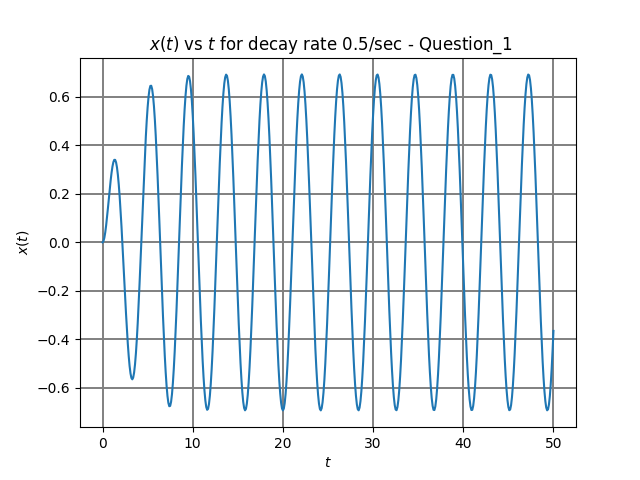
\includegraphics[scale=0.5]{figure0.png}
   	\label{fig:32}
   \end{figure}
\begin{figure}[!tbh]
   	\centering
   	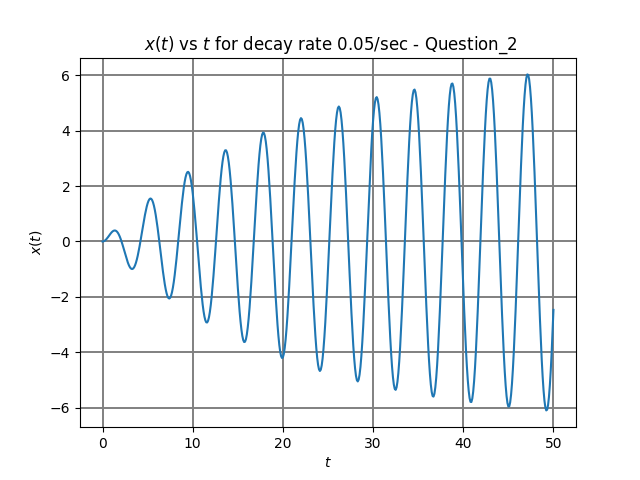
\includegraphics[scale=0.5]{figure1.png}
   	\label{fig:32}
   \end{figure}
{
We observe that the osciallation amplitude settles to  a fixed value in both the cases.
We observe it takes longer to settle with decay being less.
We also observe that the amplitude increases to a much larger amount in the case with lower decay.
At zero (or negative) decay the amplitude increases ad infinitum, and at high decay it reaches the max amplitude almost instantaneously.
}
\subsubsection{Varying the frequency of the input}
{
We vary the frequency of the cosine  and see what affect it has on the output.
We also construct the bode plot of the transfer function to better understand the results. 
}

\begin{figure}[!tbh]
   	\centering
   	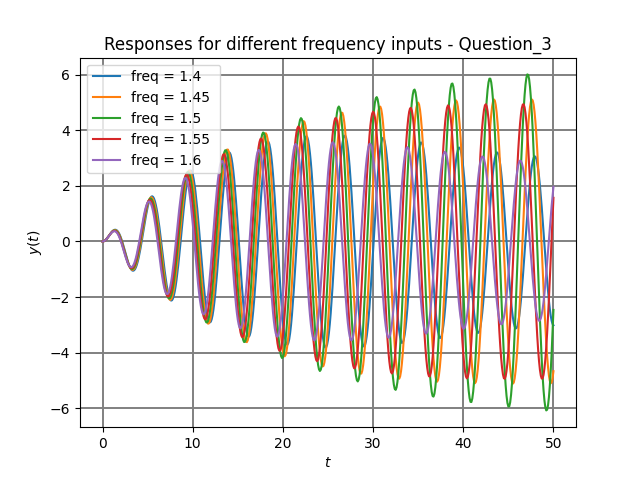
\includegraphics[scale=0.5]{figure2.png}
   	\label{fig:32}
   \end{figure}

When the input frequency is at the natural frequency the output amplitude is maximum.
In the other cases the output amplitude decreases.
This phenomenon is known as resonance.
We can see clear from the bode plot that there is a maximum at the natural frequency, as there is a second order pole there.
The phase shift is -180$\deg$, which agrees with the fact that the pole is in the left half plane.
}
\subsection{Coupled Spring Problem}
{
In this problem we have two differential equations and two variables to solve for.
The equations are
\[\dv[2]{x}{t} +(x-y) = 0 \]
\[\dv[2]{y}{t} +2(y-x) = 0 \]
With initial condition as x(0) = 1
We substitute for y in the second equation from the first, and we get a fourth order differential equation in terms of x.
Simplifying this and substituting to find the y equation, we get.
\[X(s) = \frac{s^2+2}{s^3+3s} \]
\[Y(s) =  \frac{2}{s^3+3s} \]
We can take the ILT of these two expressions to find the time domain expressions for x(t) and y(t).
We plot these in 1 graph.
}

\begin{figure}[!tbh]
   	\centering
   	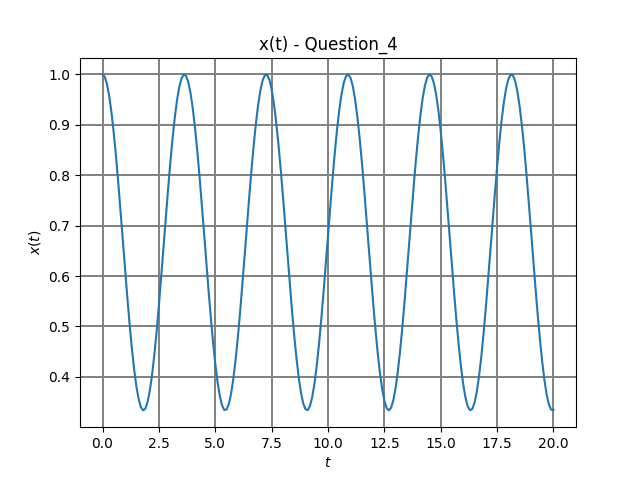
\includegraphics[scale=0.5]{figure3.png}
   	\label{fig:32}
   \end{figure}
{ 
We observe that the amplitude of y is greater than x. 
The phase of the two are opposite.
The offsets are the same for both the expressions.
This models two masses attached to the ends of an ideal spring.
}
\subsection{RLC Filter}
{
We now consider the case of an RLC Filter with the transfer function as shown.
\[ H(s) = \frac{1}{10^{-12}s^2 + 10^{-4}s + 1}\]
(Initial Conditions all zero)
The input is of the form
\[x(t) = \cos{(10^3t)}+\cos{(10^6t)} \]

which is basically the superposition of two sinusoids with low and high frequencies.
First we plot the bode plot of the transfer function.
Then we use sp.lsim to find the output of the filter to the input system.
We plot the output from 0 to 30$\mu$s as well as from 0 to 10ms.
}

\begin{figure}[!tbh]
   	\centering
   	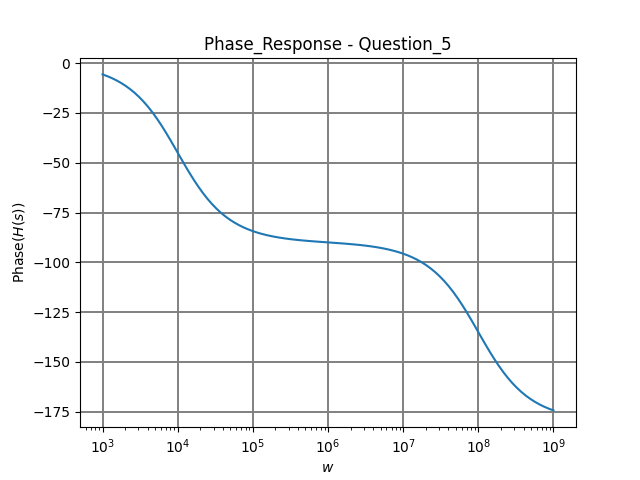
\includegraphics[scale=0.5]{figure6.png}
   	\label{fig:32}
   \end{figure}
\begin{figure}[!tbh]
   	\centering
   	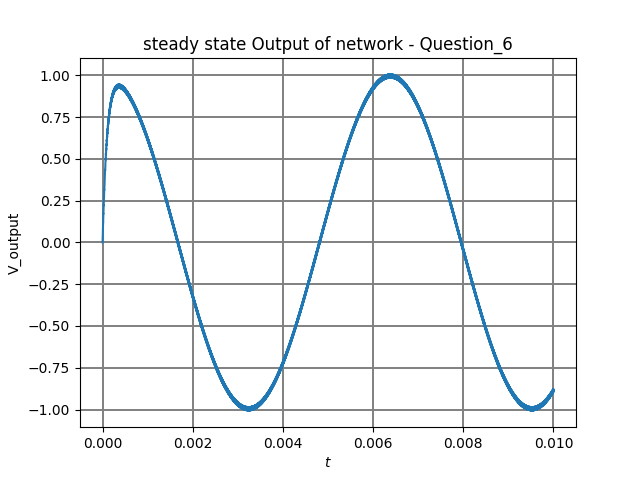
\includegraphics[scale=0.5]{figure7.png}
   	\label{fig:32}
   \end{figure}
\begin{figure}[!tbh]
   	\centering
   	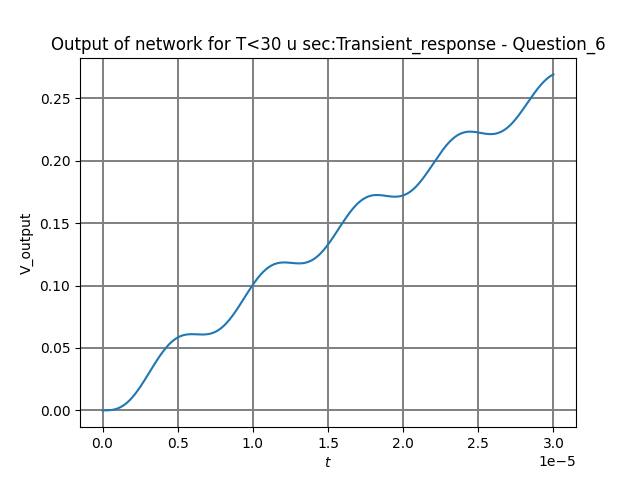
\includegraphics[scale=0.5]{figure8.png}
   	\label{fig:32}
   \end{figure}
{
From the Bode plot, it is clear that the RLC System is a second order low pass filter, with the 3db bandwidth of 
The slow time plot shows that the capacitor is charging up to meet the input amplitude. The high frequency component can be seen as a ripple in the slow time plot.  This component is highly attenuated and hence not visible in the fast time plot.
In the fast time plot, we see that the low frequency component passes almost unchanged, the amplitude is almost 1.
The reason is that the $\omega = 10^3\frac{rad}{s}$ is well within the 3-dB bandwidth ($\omega_{3dB} = 10^4\frac{rad}{s}$) of the system.
Clearly this reiterates the fact that this is a low pass filter with bandwidth $\omega_{3dB} = 10^4\frac{rad}{s}$.

}

\section{Conclusions}
The ripple in the signal in small time interval plot is because of the high frequency component. But the ripples
are not visible in large time interval because the presence of low frequency component of which amplitude
remained almost unchanged and dominated high frequency signal.
\end{document}
